\documentclass{article}
\usepackage[x11names, rgb]{xcolor}
\usepackage[utf8]{inputenc}
\usepackage{tikz}
\usetikzlibrary{snakes,arrows,shapes}
\usepackage{amsmath}
%
%

%

%

\begin{document}
\pagestyle{empty}
%
%
%

\enlargethispage{100cm}
% Start of code
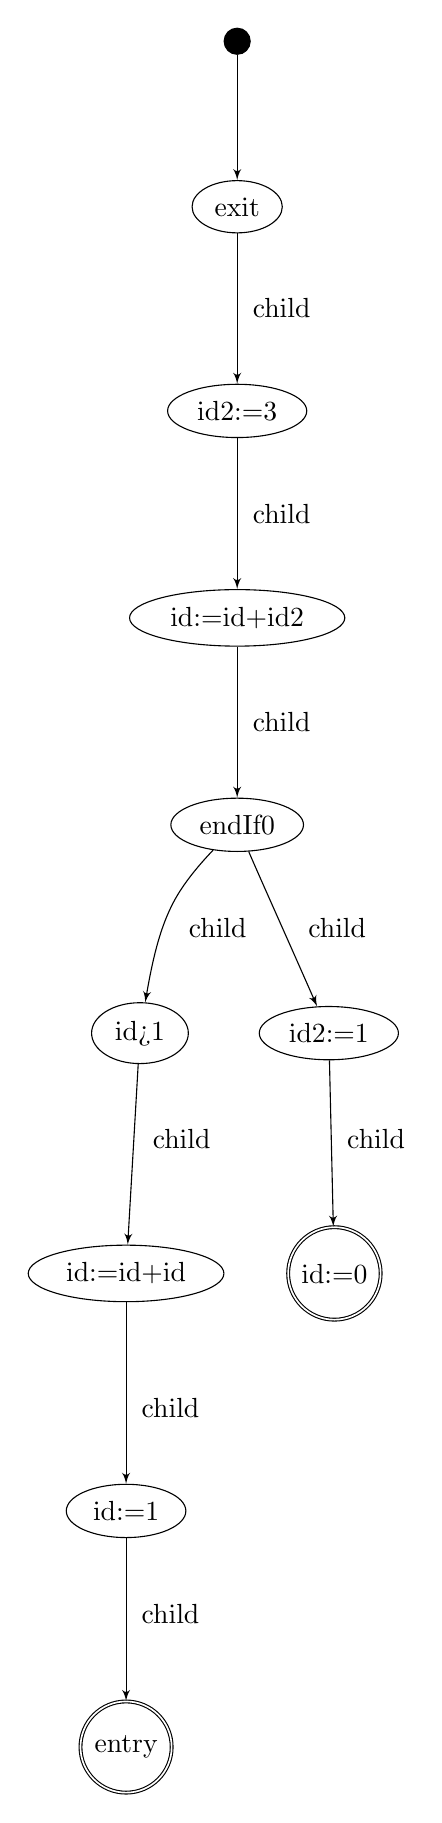
\begin{tikzpicture}[>=latex',line join=bevel,]
%%
\node (inic) at (75.5bp,635.08bp) [draw,circle, fill] {};
  \node (exit) at (75.5bp,575.5bp) [draw,ellipse] {exit};
  \node (entry) at (35.5bp,21.0bp) [draw,circle, double] {entry};
  \node (n0) at (35.5bp,106.0bp) [draw,ellipse] {id:=1};
  \node (n1) at (35.5bp,191.5bp) [draw,ellipse] {id:=id+id};
  \node (n2) at (110.5bp,191.5bp) [draw,circle, double] {id:=0};
  \node (n3) at (108.5bp,278.0bp) [draw,ellipse] {id2:=1};
  \node (n4) at (40.5bp,278.0bp) [draw,ellipse] {id>1};
  \node (n5) at (75.5bp,353.0bp) [draw,ellipse] {endIf0};
  \node (n6) at (75.5bp,427.5bp) [draw,ellipse] {id:=id+id2};
  \node (n7) at (75.5bp,502.0bp) [draw,ellipse] {id2:=3};
  \draw [->] (n5) ..controls (61.535bp,338.32bp) and (56.028bp,331.77bp)  .. (52.5bp,325.0bp) .. controls (48.31bp,316.96bp) and (45.506bp,307.35bp)  .. (n4);
  \definecolor{strokecol}{rgb}{0.0,0.0,0.0};
  \pgfsetstrokecolor{strokecol}
  \draw (68.5bp,316.0bp) node {child};
  \draw [->] (exit) ..controls (75.5bp,555.02bp) and (75.5bp,536.59bp)  .. (n7);
  \draw (91.5bp,539.0bp) node {child};
  \draw [->] (n3) ..controls (108.96bp,257.44bp) and (109.39bp,239.51bp)  .. (n2);
  \draw (125.5bp,240.0bp) node {child};
  \draw [->] (n6) ..controls (75.5bp,405.62bp) and (75.5bp,387.24bp)  .. (n5);
  \draw (91.5bp,390.0bp) node {child};
  \draw [->] (n0) ..controls (35.5bp,85.375bp) and (35.5bp,67.833bp)  .. (entry);
  \draw (51.5bp,69.0bp) node {child};
  \draw [->] (inic) ..controls (75.5bp,614.16bp) and (75.5bp,604.05bp)  .. (exit);
  \draw [->] (n7) ..controls (75.5bp,480.99bp) and (75.5bp,462.69bp)  .. (n6);
  \draw (91.5bp,465.0bp) node {child};
  \draw [->] (n4) ..controls (39.113bp,253.56bp) and (37.688bp,229.48bp)  .. (n1);
  \draw (55.5bp,240.0bp) node {child};
  \draw [->] (n1) ..controls (35.5bp,167.64bp) and (35.5bp,143.33bp)  .. (n0);
  \draw (51.5bp,143.0bp) node {child};
  \draw [->] (n5) ..controls (84.643bp,331.77bp) and (93.529bp,312.12bp)  .. (n3);
  \draw (111.5bp,316.0bp) node {child};
%
\end{tikzpicture}
% End of code

%
\end{document}
%



